\chapter{Introduction à l'optimisation}
%\addcontentsline{toc}{chapter}{TD 1}

\section{Questions de cours}

\begin{enumerate}
	\item On considère le problème \eqref{eq:pb-optim} d'optimisation suivant:
	\eq{\label{eq:pb-optim}\tag{$\Pp$}
		\min_{x_1,x_2} (x_1 - 3)^2 + (x_2 + 2)^2 \qtqq
		\left\{ \begin{aligned}
			& 3x_2^2 - x_2 = 0\\
			& x_1 + x_2 \leq 2
		\end{aligned} \right. 
	}
	\begin{enumerate}
		\item Donner la ou les variables du problème \eqref{eq:pb-optim}. Quelle est la dimension de ce problème?
		\item Donner l'expression de la fonction objectif du problème \eqref{eq:pb-optim}.
		\item Donner les contraintes du problème \eqref{eq:pb-optim} et les classer par catégorie.
		\item A partir de votre analyse du problème \eqref{eq:pb-optim}, proposer une simplification sous la forme d'un nouveau problème d'optimisation équivalent.
	\end{enumerate}
	
	\item On considère à présent le problème d'optimisation suivant:
	\eq{
		\min_{x_1,x_2} 100(x_2 - x_1^2)^2 + (1-x_1)^2
	}
	\begin{enumerate}
		\item Caractériser le problème d'optimisation: variables, fonction objectif, contraintes.
		\item Soit $\bm{x}^\star \in \RR^2$. Enoncer une condition nécessaire pour que $\bm{x}^\star$ soit un minimiseur local du problème d'optimisation.
		\item Le vecteur $(0,0)^\top$ est-il un minimiseur local du problème?
	\end{enumerate}
\end{enumerate}


\section{Formulation d'un problème d'optimisation}

Des manufactures livrent chaque matin des pièces de carrosserie dans des usines d'assemblage de voitures. Il y a $n$ manufactures qui produisent chacune une quantité journalière (fixe) $a_1, \ldots, a_n$ de pièces, et $m$ usines qui ont un besoin quotidien (fixe) de $b_1, \ldots, b_m$ pièces, respectivement. On suppose que la quantité totale produite est égale à la quantité totale requise: les manufactures doivent écouler toutes leurs pièces, les usines doivent recevoir toutes leurs pièces.

Chaque manufacture peut livrer à plusieurs usines. La livraison de la $i$-ème manufacture vers la $j$-ème usine coûte $c_{ij}$. On souhaite déterminer le plan de livraison optimal, c'est-à-dire le nombre $p_{ij}$ de pièces que chaque manufacture $i$ doit expédier à chaque usine $j$ de manière à minimiser le coût total des livraisons.

\begin{enumerate}
	\item Quelles sont les variables de ce problème d'optimisation?
	\item Exprimer la fonction objectif du problème en fonction de l'ensemble des coûts $c_{ij}$
	\item Quelles sont les contraintes du problème? Ecrire le problème d'optimisation final.
\end{enumerate}

\begin{hide}
\paragraph{\textcolor{blue}{Solution.}} 
\begin{enumerate}
	\item Les variables du problème sont les quantités que l'on souhaite optimiser, cad ici les $p_{ij}$. Toutes les autres grandeurs ($a_i$, $b_j$, $c_{ij}$) sont des données du problème.

	\item L'envoi de $p_{ij}$ pièces de la manufacture $i$ vers l'usine $j$ coûte $p_{ij} \cdot c_{ij}$. La fonction objectif du problème, c'est-à-dire le coût total de tous les envois, est donc
\eq{
	f(P) = \sum_{i=1}^n \sum_{j=1}^m c_{ij} \cdot p_{ij} = \Tr(C P)
}
où $C$ est la matrice de coût, et $P$ est la matrice des $p_{ij}$, (appelée \textit{plan de transport}).

	\item La première contrainte est que les manufactures doivent écouler toutes leurs pièces dans les usines: il faut donc que pour toute manufacture $i$, $a_i = \sum_{j=1}^m p_{ij}$ (certains $p_{ij}$ peuvent bien sûr valoir $0$). 
	
	De même, les usines doivent recevoir toutes leurs pièces depuis les manufactures: pour tout $j$, il faut $b_j = \sum_{i=1}^n p_{ij}$.
	
	Le problème d'optimisation final s'écrit donc:
	\eq{
		\min_{p_{ij}} \sum_{i=1}^n  \sum_{j=1}^m c_{ij} p_{ij} \qscq 
		\left\{\begin{aligned}
			&\sum_{j=1}^m p_{ij} = a_i \quad \forall i=1,\ldots,n\\
			&\sum_{i=1}^m p_{ij} = b_j \quad \forall j=1,\ldots,m\\
		\end{aligned}\right.
	}
	Ce problème peut aussi s'écrire de manière plus condensée en fonction des matrices:
	\eq{
		\min_{P \in \RR^{n\times m}} \Tr(CP) \qscq
		\left\{\begin{aligned}
			&P \mathds{1} = a\\
			&P^\top \mathds{1} = b
		\end{aligned}\right.
	}
	où $\mathds{1} = (1,1,\ldots,1)^\top$.
\end{enumerate}
\end{hide}


\section{Calcul vectoriel}
Pour chacune des fonctions suivantes, calculer le gradient et la Hessienne:
\begin{enumerate}
	\item $f:\RR^2 \to \RR, \quad f(x) = x_1^3 - 2x_2^2 + 6x_1 - 24$.
	\item $f:\RR^2 \to \RR, \quad f(x) = 100(x_2 - x_1^2)^2 + (1-x_1)^2$.
	\item $f:\RR^3 \to \RR, \quad f(x) = x^\top Q x + b^\top x$, où $Q \in \RR^{3\times 3}$ et $b \in \RR^3$.
\end{enumerate}

\section{Convexité}
\begin{enumerate} 
	\item Soit $f:\RR^n \to \RR$ une fonction. Donner la définition de la convexité de $f$. Expliquer pourquoi la convexité est une propriété intéressante en optimisation numérique.
	\item Montrer que la fonction $x \mapsto \norm{Ax}^2$, où $x\in \RR^3$ et $A \in \RR^{3\times 3}$, est convexe.
	\item Parmi les fonctions univariées suivantes, lesquelles sont convexes?
	
	\begin{figure}[h]
		\subfloat[]{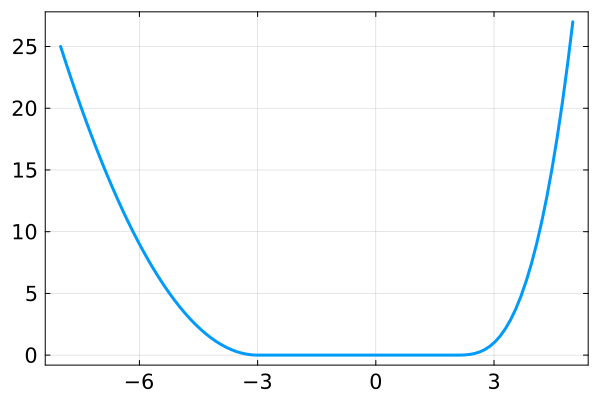
\includegraphics[width=0.3\textwidth]{td1/plots-td1-exemple1}}
		\hfill
		\subfloat[]{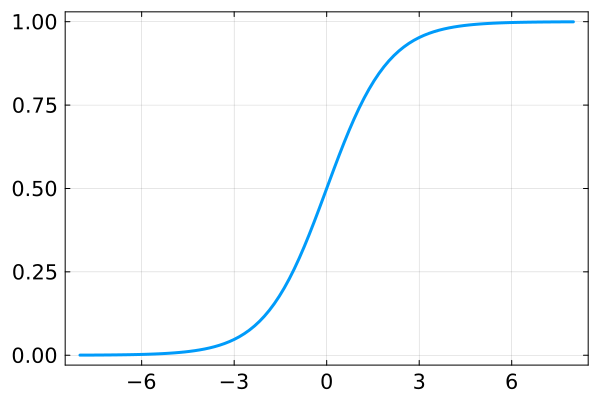
\includegraphics[width=0.3\textwidth]{td1/plots-td1-exemple2}}
		\hfill
		\subfloat[]{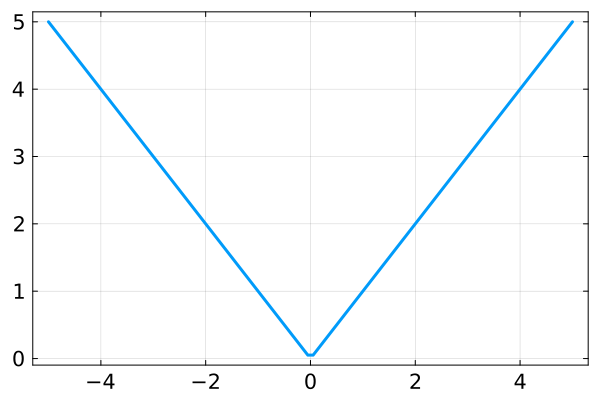
\includegraphics[width=0.3\textwidth]{td1/plots-td1-exemple3}}
	\end{figure}
	
	\item Parmi les fonctions bivariées suivantes, lesquelles sont convexes?
	\begin{figure}[h]
		\subfloat[]{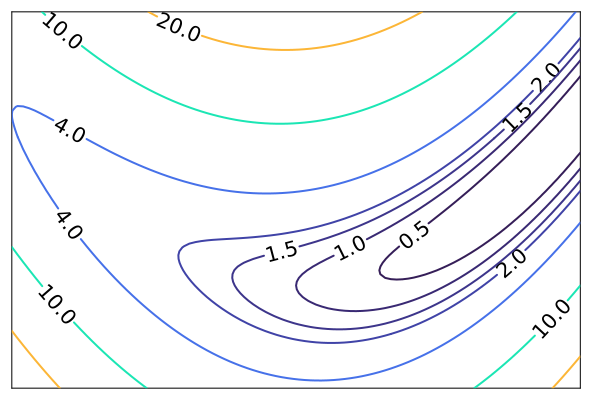
\includegraphics[width=0.3\textwidth]{td1/plots-td1-Rosenbrock}}
		\hfill
		\subfloat[]{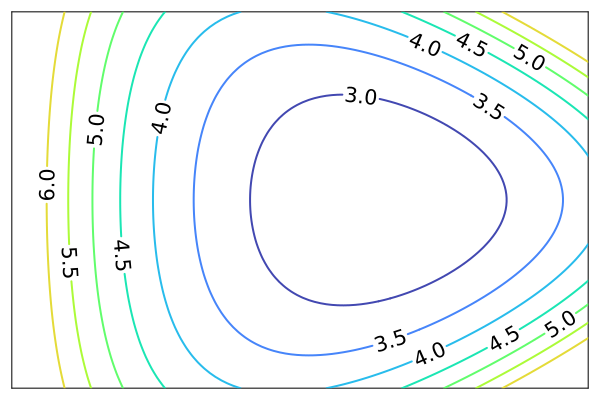
\includegraphics[width=0.3\textwidth]{td1/plots-td1-exp}}
		\hfill
		\subfloat[]{
\includegraphics[width=0.3\textwidth]{td1/plots-td1-Rastrigin}}
	\end{figure}
\end{enumerate}

\begin{hide}
\paragraph{\textcolor{blue}{Solution.}} 
\begin{enumerate}
	\item[2.] La Hessienne de $x \mapsto \norm{Ax}^2$ est $H = A^\top A$. On vérifie que $H$ est semi-définie positive: en effet, pour tout $x$,
	\eq{
		x^\top A^\top A x = \norm{Ax}^2 \geq 0.
	}
	Donc la fonction est convexe.
	\item[4.] (a) Fonction de Rosenbrock, $f(x_1,x_2) = (1-x_1)^2 + 10 * (x_2 -x_1^2)^2$. La fonction n'est pas convexe. Mais elle est convexe en $x_2$.
	
	(b) Convexe
	
	(c) Fonction de Rastrigin, pas convexe.
\end{enumerate}
\end{hide}
